\chapter{ANTECEDENTES Y ESTADO DEL ARTE}
\label{ch:2}
% ==============================================================================================================
\section{Introducción}

En esta sección se encuentra en una frontera muy difusa de multiples ramas del conocimiento, siendo muy interdisciplinar, se trata de una revisión de los ataques, seguridad y robustez a las redes neuronales.
Por lo que debemos explicar que es la ciencia de datos, el proceso \gls{KDD}, la inteligencia artifical generativa y los posibles

\begin{figure}[H]
  \centering
  \centerline{\includesvg[width=0.75\columnwidth]{figures/ciencia-de-datos.drawio.svg}}
  \caption{Ciencia de datos como campo interdisciplinar.\\Fuente: Elaboración propia}
  \label{fig:ciencia-de-datos}
\end{figure}

Podemos dividir este trabajo en dos secciones muy relacionadas, la primera la inteligencia artificial y como segundo punto de importancia la seguridad.
Desde sus inicios la inteligencia artificial aunque con buenos resultados en muchos campos de aplicación resulaba en grandes fallos de seguridad, fiabilidad y robustez.
Por como están entrenadas las inteligencias artificiales (\acrshort{nn}) tiene multiples puntos de ataque que son susceptibles de ser atacados, los principales son los datos, las arquitecturas o los pesos.
Ya que alterando cualquiera de estos componentes de forma se verá enormemente afectada el comportamiento.

% Ciencia de la computación
% Mineria
% Machine Learning
% Deep Learning
% GANs


\section{Antecedentes}


\subsection{Historia, línea temporal}

A continuación se describe una línea de temporal con los hitos más relevantes en el desarrollo de las redes neuronales adjuntando con referencias las investigaciones, articulos y publicaciones realizadas.
En este caso se trata de referencias en hitos de logros a nivel teórico como práctico.

\begin{vtimeline}[timeline color=cyan!80!blue, add bottom line, line offset=2pt, use timeline header,timeline title={Hitos de las redes neuronales artificiales}]
  1676        & The Chain Rule \cite{leibniz2012early}                                                    \endlr
  1847        & Augustin-Louis Cauchy \cite{lemarechal2012cauchy}                                         \endlr
  1943        & Threshold Logic Unit (TLU) \cite{mcculloch1943logical}                                    \endlr
  1949        & Teoría Hebbiana                                                                           \endlr
  1958        & Perceptron \cite{rosenblatt1958perceptron}                                                \endlr
  1959-1960   & Adaline y Madaline \cite{rosenblatt1958perceptron}                                        \endlr
  1965        & Multilayer Perceptron (MLP) \cite{baum1988capabilities}                                   \endlr
  1967-1968   & Deep Learning by Stochastic Gradient Descent \cite{karplus19671967}                       \endlr
  1980’s      & Neuronas Sigmoidales                                                                      \endlr
  ~           & Feedforward neural network (FNN) \cite{rumelhart1985learning}                             \endlr
  ~           & Backpropagation (BP) \cite{rosenblatt1962principles,etde_5080493,lecun1985learning}       \endlr
  1985        & Boltzmann Machine \cite{ACKLEY1985147}                                                    \endlr
  1987        & Adaptive resonance theory (ART) \cite{grossberg1987competitive}                           \endlr
  1989        & Convolutional neural networks (CNN) \cite{lecun1989backpropagation}                       \endlr
  ~           & Recurent neural networks (RNN) \cite{schmidhuber1993habilitation}                         \endlr
  1990        & Generative Adversarial Networks (GAN) as Game \cite{schmidhuberunsupervised}              \endlr
  1997        & Long short term memory (LSTM) \cite{Hochreiter1997LongSM, hochreiter1997long}                                 \endlr
  2006        & Deep Belief Networks (DBN) \cite{hinton2006fast}                                          \endlr
  ~           & Restricted Boltzmann Machine \cite{hinton2006reducing}                                    \endlr
  ~           & Encoder / Decoder (Auto-encoder) \cite{hinton2006reducing}                                \endlr
  2014        & Generative Adversarial Networks (GAN) Moderns \cite{6294131,goodfellow2014generative}     \endlr
  2018        & Style Generative Adversarial Networks (Style-GAN) \cite{karras2019stylebased}             \endlr
\end{vtimeline}


\newpage
\subsection{Historia de la Inteligencia Artificial}

% \begin{wrapfigure}{R}{0.25\textwidth}
%     \vspace{-20pt}
%     \begin{center}
%         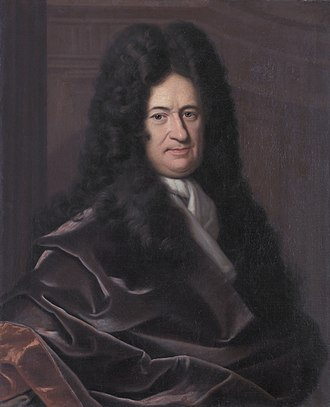
\includegraphics[width=0.25\textwidth]{figures/Gottfried_Wilhelm_Leibniz,_Bernhard_Christoph_Francke.jpg}
%         \label{fig:Gottfried-Leibniz}
%     \end{center}
%     \caption{Retrato de Gottfried Leibniz, por Christoph Bernhard Francke. \\Fuente: \href{https://es.wikipedia.org/wiki/Gottfried_Leibniz}{Wikipedia}}
%     \vspace{-20pt}
% \end{wrapfigure}

Todo surge en 1676 por {Gottfried Wilhelm Leibniz} \ref{fig:gottfried-leibniz} publicó la regla de la cadena del cálculo diferencial, esencial para el análisis matemático, es la esencial para calcular como cambiará la función final si se cambian los pesos de funciones anteriores.

La regla de la cadena es fundamental para técnicas como el descenso de gradiente, propuesto por {Augustin-Louis Cauchy} en 1847 y utilizado para ajustar iterativamente los pesos de una NN durante el entrenamiento.
Posteriormente en 1805 {Adrien-Marie Legendre} y {Johann Carl Friedrich Gauss} desarrollaron \acrshort{nn}, matemáticamente eran regresiones lineales muy simples, similares a las redes neuronales lineales simples.
Esto lo uso {Gauss} para redescubrir el planeta enano Ceres.

\begin{figure}[H]
  \centering
  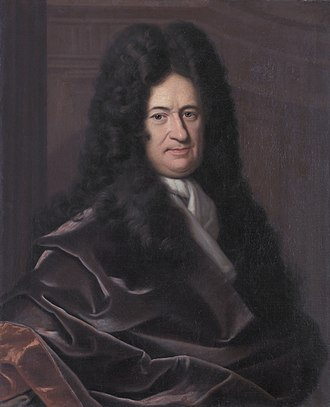
\includegraphics[width=0.45\textwidth]{figures/Gottfried_Wilhelm_Leibniz,_Bernhard_Christoph_Francke.jpg}
  \caption{Retrato de Gottfried Leibniz. \\Fuente: \href{https://es.wikipedia.org/wiki/Gottfried_Leibniz}{Wikipedia}}
  \label{fig:gottfried-leibniz}
\end{figure}

Aunque realmente la historia comienza en 1943 con la investigación de {Warren McCulloch} y {Walter Pitss}, publicaron el artículo \textit{A logical calculus of the ideas immanent in nervous activity} \cite{mcculloch1943logical}.
Dicho artículo creó distintas ramas de investigación (ordenadores digitales, inteligencia artificial, funcionamiento del perceptron).

\begin{figure}[H]
  \centering
  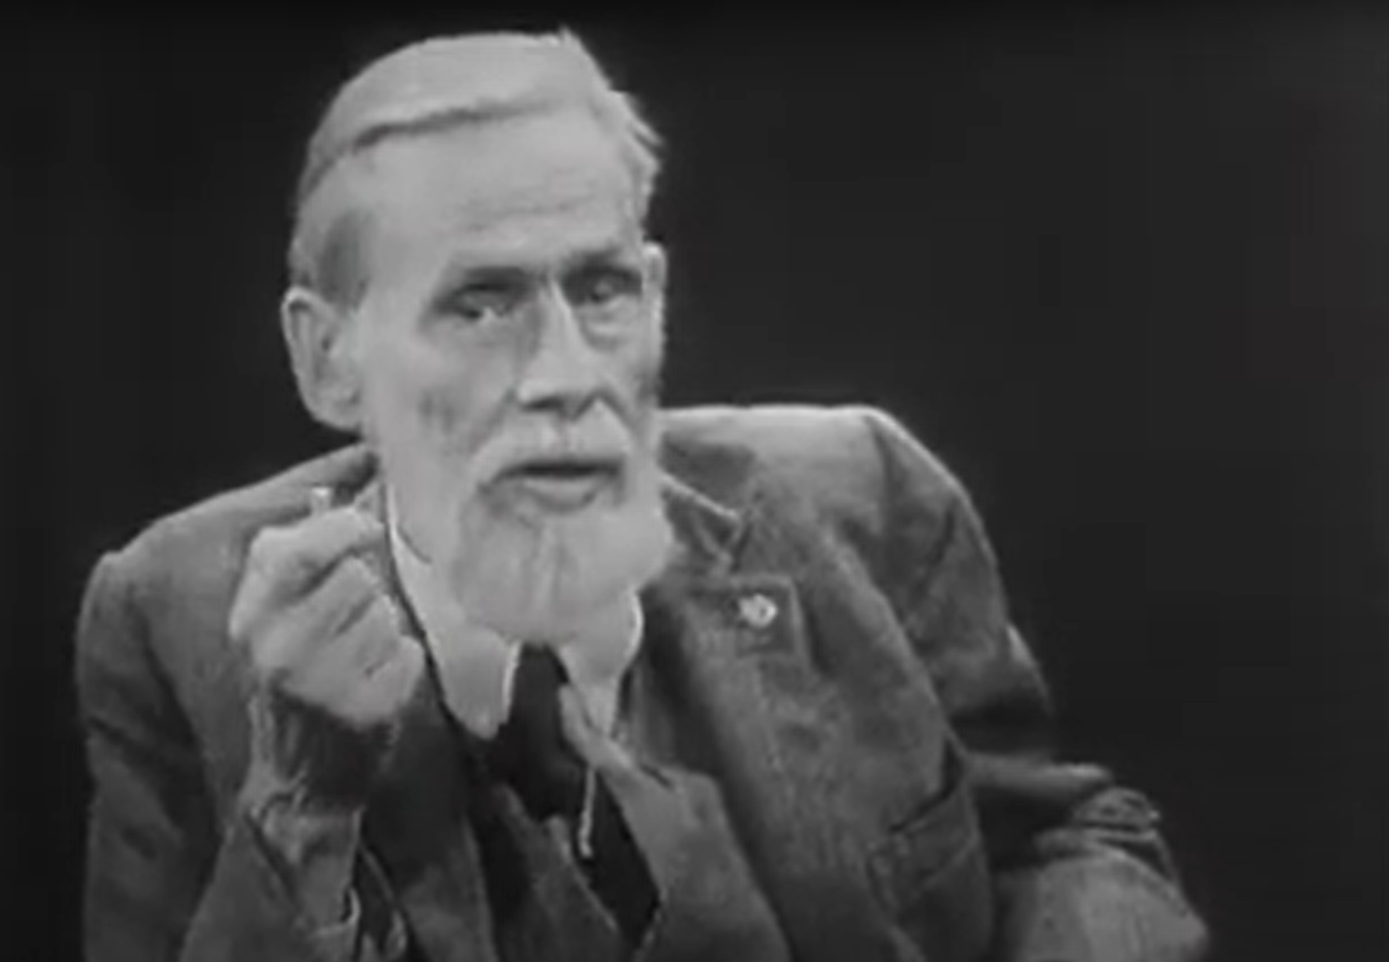
\includegraphics[width=0.65\textwidth]{figures/Warren Sturgis McCulloch Interview.png}
  \caption{Warren Sturgis McCulloch Interview. \\Fuente: \href{https://www.youtube.com/watch?v=8Wdz1Tj5084}{Entrevista en 1969}}
  \label{fig:Warren Sturgis McCulloch}
\end{figure}


En 1956 en la primera conferencia de inteligencia artificial organizada por la fundación {Rochester}, se reunen los investigadores fundadores de los conceptos actuales de la IA ({Minsky, McCarthy, Rochester, Shanon}), gran parte de la bibliografia se refiere a este punto como el origen y contacto de las redes neuronales artificiales.
En dicha conferencia (\textit{Nathaural Rochester}) presento el modelo de una red neuronal que fue el resultado de la investigación desarrollada por el equipo de investigación de IBM.

\begin{figure}[H]
  \centering
  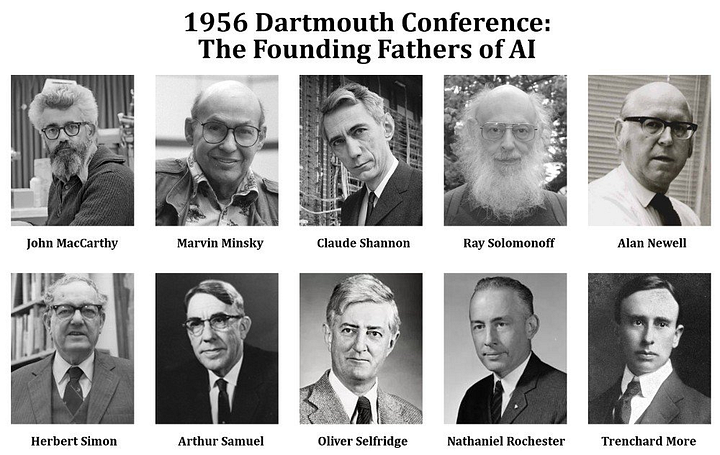
\includegraphics[width=0.75\textwidth]{figures/conferecia 1956 - 1689170718524.png}
  \caption{Los padres de la inteligencia artificial. \\Fuente: \href{https://www.linkedin.com/pulse/first-ever-ai-conference-tracing-evolution-history-ofai-nicky-verd}{Linkedin}}
  \label{fig:conferencia-1956}
\end{figure}

En 1957 se presenta el ``Perceptron'' por {Frank Rosenblatt}, dicho elemento es un sistema clasificador de patrones, además contaba con la capacidad de aprender, de ser robusto matemáticamente y poder adaptarse si algún componente se dañaba.

\begin{figure}[H]
  \centering
  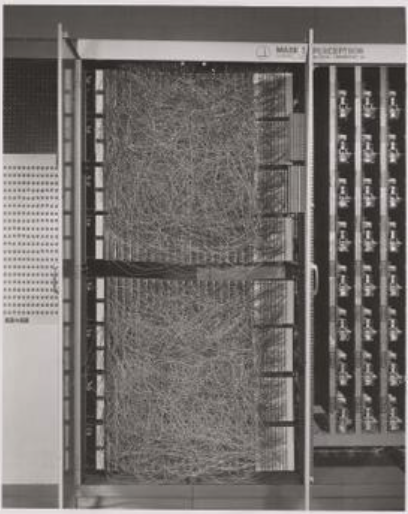
\includegraphics[width=0.4\textwidth]{figures/perceptron.png}
  \caption{Mark I Perceptron. \\Fuente: \href{https://en.wikipedia.org/wiki/Perceptron}{Wikipedia}}
  \label{fig:perceptron}
\end{figure}

El Perceptron fue diseñado originalmente para el reconocimiento óptico usando un sistema de 400 fotocélulas en rejilla, también se describio el problema de no-linealidad que presentaban los perceptrones (Problema XOR) \cite{cuevastello2018apuntes}.

De 1959 a 1960 {Bernard Widrow} y {Ted Hoff} desarollaron ``Adaline'' y ``Madaline'' \cite{widrow1960adaptive} que resolvia el problema de la no-linealidad y que tenía aplicación en el reconocimiento de voz, series temporales, carácteres, etc.

Posteriormente el MIT realizo una investigación mátematica muy crítica de todos los problemas que presentaba el Perceptron llegando a la conclusión que tenian grandes problemas que no podrian ser resueltos, por lo que en la proxima década (años 60) se redujo drasticamente las investigaciones sobre el campo de las redes neuronales.
Esto llevo a uno de los famosos inviernos de la inteligencia artificial (1974 - 1980).


% \begin{wrapfigure}{R}{0.25\textwidth}
%     \vspace{-20pt}
%     \begin{center}
%         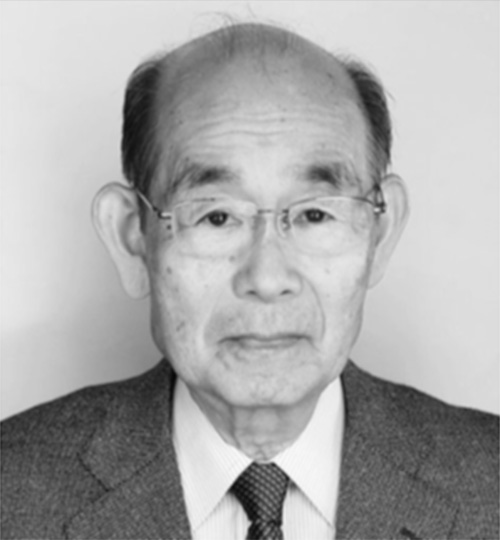
\includegraphics[width=0.25\textwidth]{figures/Kunihiko Fukushima.jpg}
%         \label{fig:kunihiko-fukushima}
%     \end{center}
%     \vspace{-20pt}
%     \caption{Kunihiko Fukushima. \\Fuente: \href{https://www.ieice.org/eng/about_ieice/new_honorary_members_award_winners/2017/meiyo_05e.html}{IEICE}}
% \end{wrapfigure}

\begin{figure}[H]
  \centering
  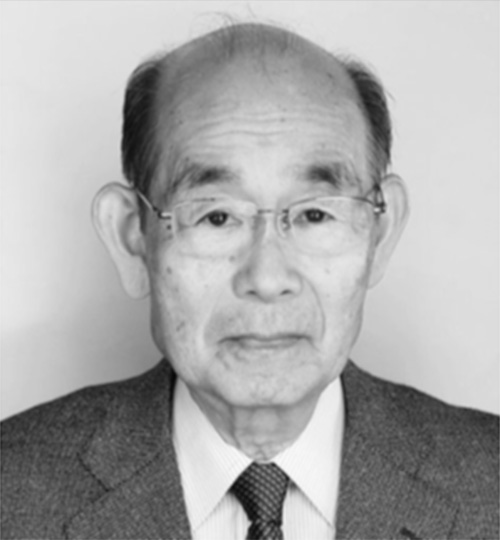
\includegraphics[width=0.25\textwidth]{figures/Kunihiko Fukushima.jpg}
  \caption{Kunihiko Fukushima. \\Fuente: \href{https://www.ieice.org/eng/about_ieice/new_honorary_members_award_winners/2017/meiyo_05e.html}{IEICE}}
  \label{fig:kunihiko-fukushima}
\end{figure}

Durante la década de los 70 se hacen aportes a la teoría Hebbiana, se aportan logros en al análisis y descripción de reglas adaptativas, además de otros aportes al principio de aprendizaje competitivo.
En 1979 presentó {Kunihiko Fukushima} la primera red neuronal \acrshort{cnn}, la llamó Neocognitron \cite{fukushima1979neural}, dicho trabajo en un futuro se mejoraría con técnicas de \gls{BP-NN}.


En la década de los 80 se realizaron aportes como el algoritmo de \gls{BP-NN} que surgio del artículo de {Hopfield} \cite{hopfield1982neural}, esto despertó la curiosidad de muchos investigadores a volver al campo de las redes neuronales.
Se realizaron aportes como las redes \acrshort{gnn}.
La investigación continuó con {Stephen Grossberg} que realizo aportes derivados de estudios fisiológicos de como funcionaban las neuronas y la plasticidad, lo que permitio la creación de reglas y postulados, esto se ve en los trabajos de las redes \acrshort{art-nn} \cite{grossberg1987competitive}.
La investigación de {Hopfield} basada en el trabajo de {Stephen Grossberg} creo un sistema computacional neuronal interconectado que tiende a un mínimo de energia.
En 1985 {David E. Rumelhart} basandose en la investigación realizada por {Paul Werbos} \cite{etde_5080493} realizo un análisis experimental del algoritmo \gls{BP-NN} y su aplicación en redes \acrshort{fnn} \cite{rumelhart1985learning}.

{Yann LeCun} junto a su equipo, en 1989 crearon la primera aplicación \acrshort{cnn} con técnicas \acrshort{bp} dicha aplicación podia reconocer números a partir de imágenes.

\begin{figure}[H]
  \centering
  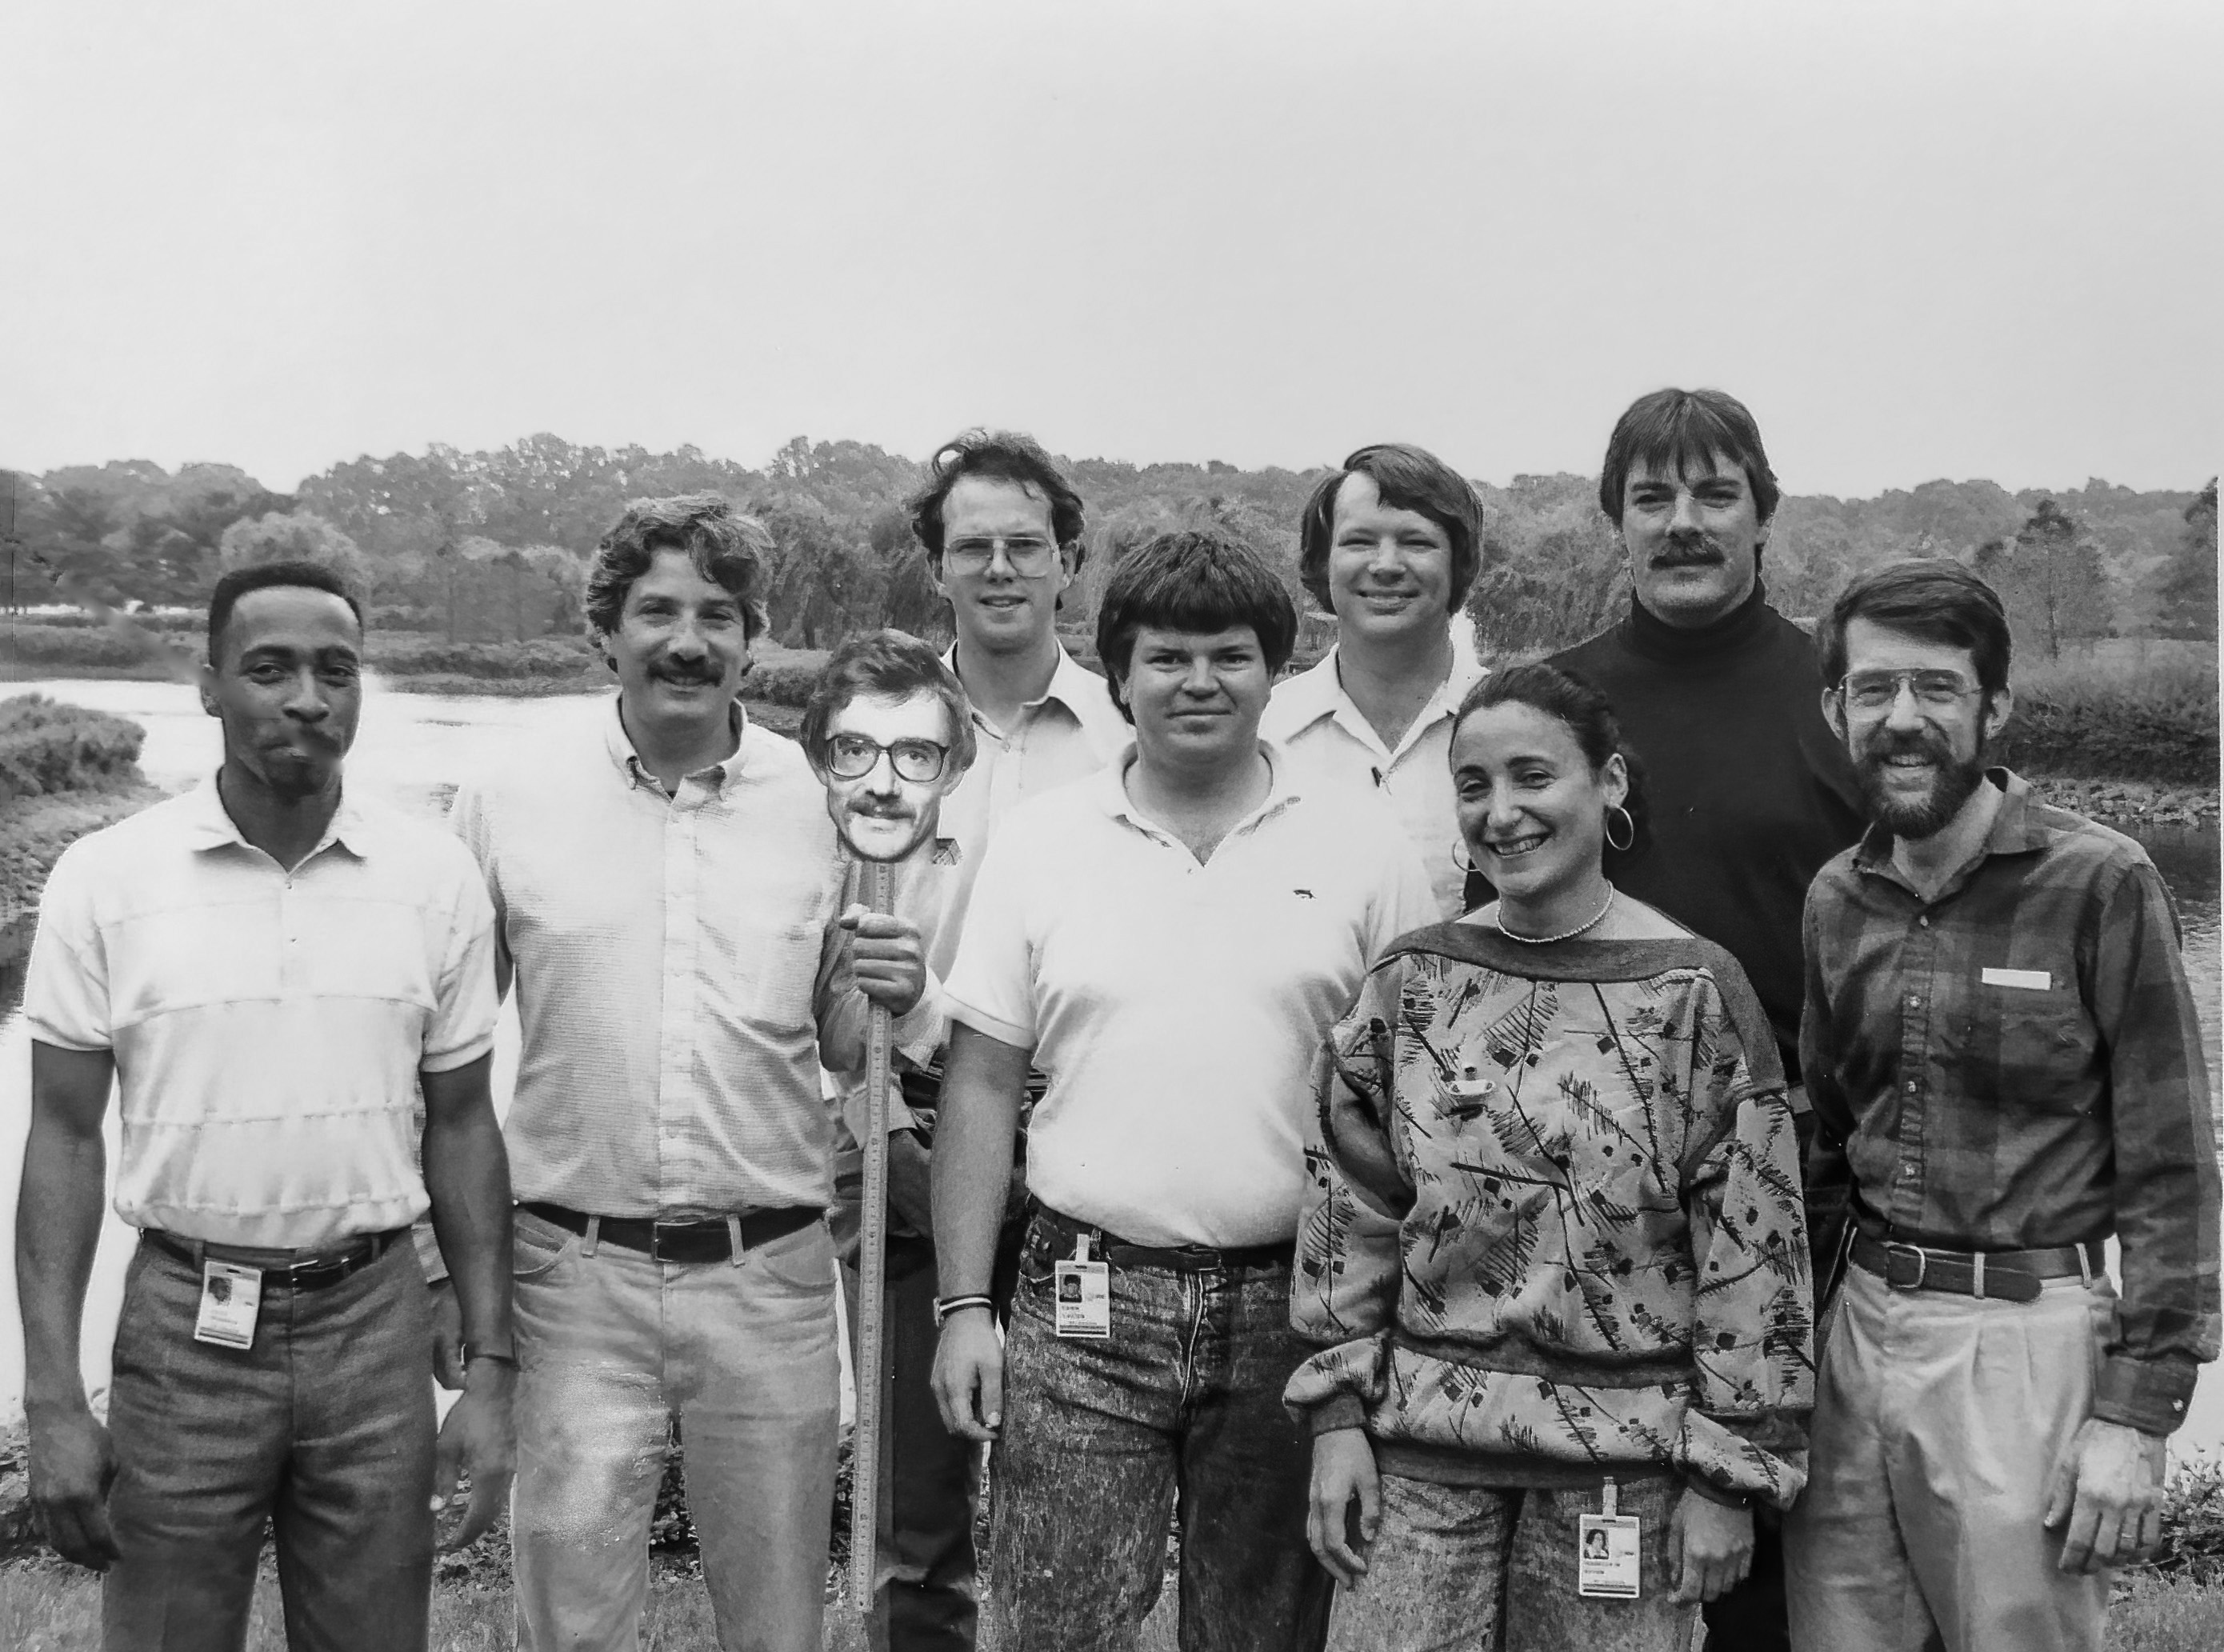
\includegraphics[width=0.65\textwidth]{figures/yann-lecun - EyIwmEDW8AIQs1C.jpeg}
  \caption{Adaptive Systems Research Department at Bell Labs 1989. \\Fuente: \href{https://twitter.com/ylecun/status/1378718317695934465}{Twitter Yann Lecun}}
  \label{fig:adaptive-systems-research-department-at-bell-labs}
\end{figure}


En la década de los 90 se presentaron multiples investigaciones y muchos avances en el campo, uno de los más importantes fue la presentación de la primera \acrshort{gan} como una curiosdidad, ya que se presentó como un duelo entre dos redes neuronales, en un principio fue un generador probabilistico y un predictor con el objetivo de maximizar la pérdida de cada uno en un juego minimax.

En 1991 se presentó el trabajo \textit{Predictability Minimization} \cite{urgen1991learning} dichas técnicas sirvieron de inspiración para el aprendizaje por refuerzo,
En marzo de 1991 se hizo una aproximación a los \textit{transformers} con auto atención, lograron separar el conocimiento del control como una máquina clásica, pero de una forma completamente neuronal, además de gestionar actualizaciones de los pesos de forma muy rápida y eficiente.

Durante la década de 1990 las redes neuronales tendian a ser muy sencillas, con pocas capas y no muy complejas por las limitaciones téncicas de la época.
Por lo que muchos investigadores propusieron soluciones similares a las redes \acrshort{rnn} que permitian una retroalimentación, además de aceptar secuencias de información arbitraria.
Otros propusieron soluciones como la jerariquia de \acrshort{rnn} autosupervisada que aprende representaciones en distintos niveles de abstraccion.
Comienzan a proponerse redes similares a las que en un futuro se llamarian \acrshort{dbn} como un método no supervisado para \acrshort{fnn}.

En junio de 1991 {Sepp Hochreiter} \ref{fig:sepp-hochreiter} implemento el primer compresor de redes neuronales, además demostró uno de los principales problemas de las \acrshort{nn} el llamado problema del desvanecimiento o explosión del gradiente que hacía que el aprendizaje fallará.
Un analisis posterior condujo a los investigadores a una primera aproximación \acrshort{lstm}, aunque no sería hasta 1997 con la revisión por pares´y publicación del artículo \textit{Long short-term memory} \cite{hochreiter1997long} que se solucionaria parcialmente el problema.
% Las \gls{RNN} se basaron en el trabajo de David Rumelhart \cite{rumelhart1985learning}

\begin{figure}[H]
  \centering
  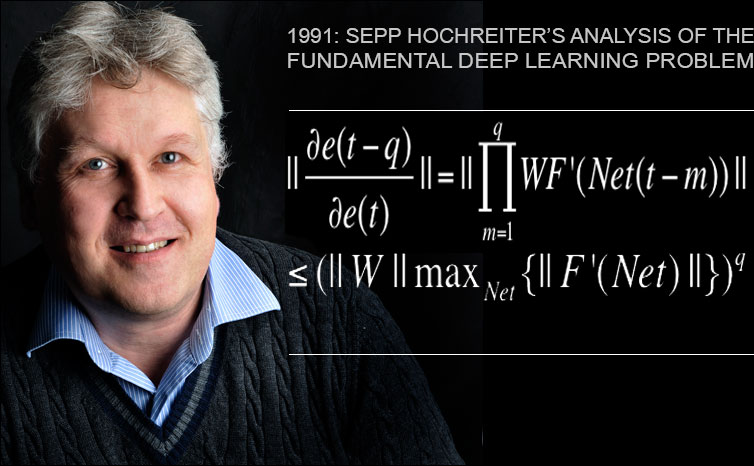
\includegraphics[width=0.65\textwidth]{figures/Sepp Hochreiter.jpg}
  \caption{Sepp Hochreiter. \\Fuente: \href{https://people.idsia.ch/~juergen/fundamentaldeeplearningproblem.html}{IDSIA}}
  \label{fig:sepp-hochreiter}
\end{figure}


% \begin{wrapfigure}{R}{0.25\textwidth}
%     \vspace{-20pt}
%     \begin{center}
%         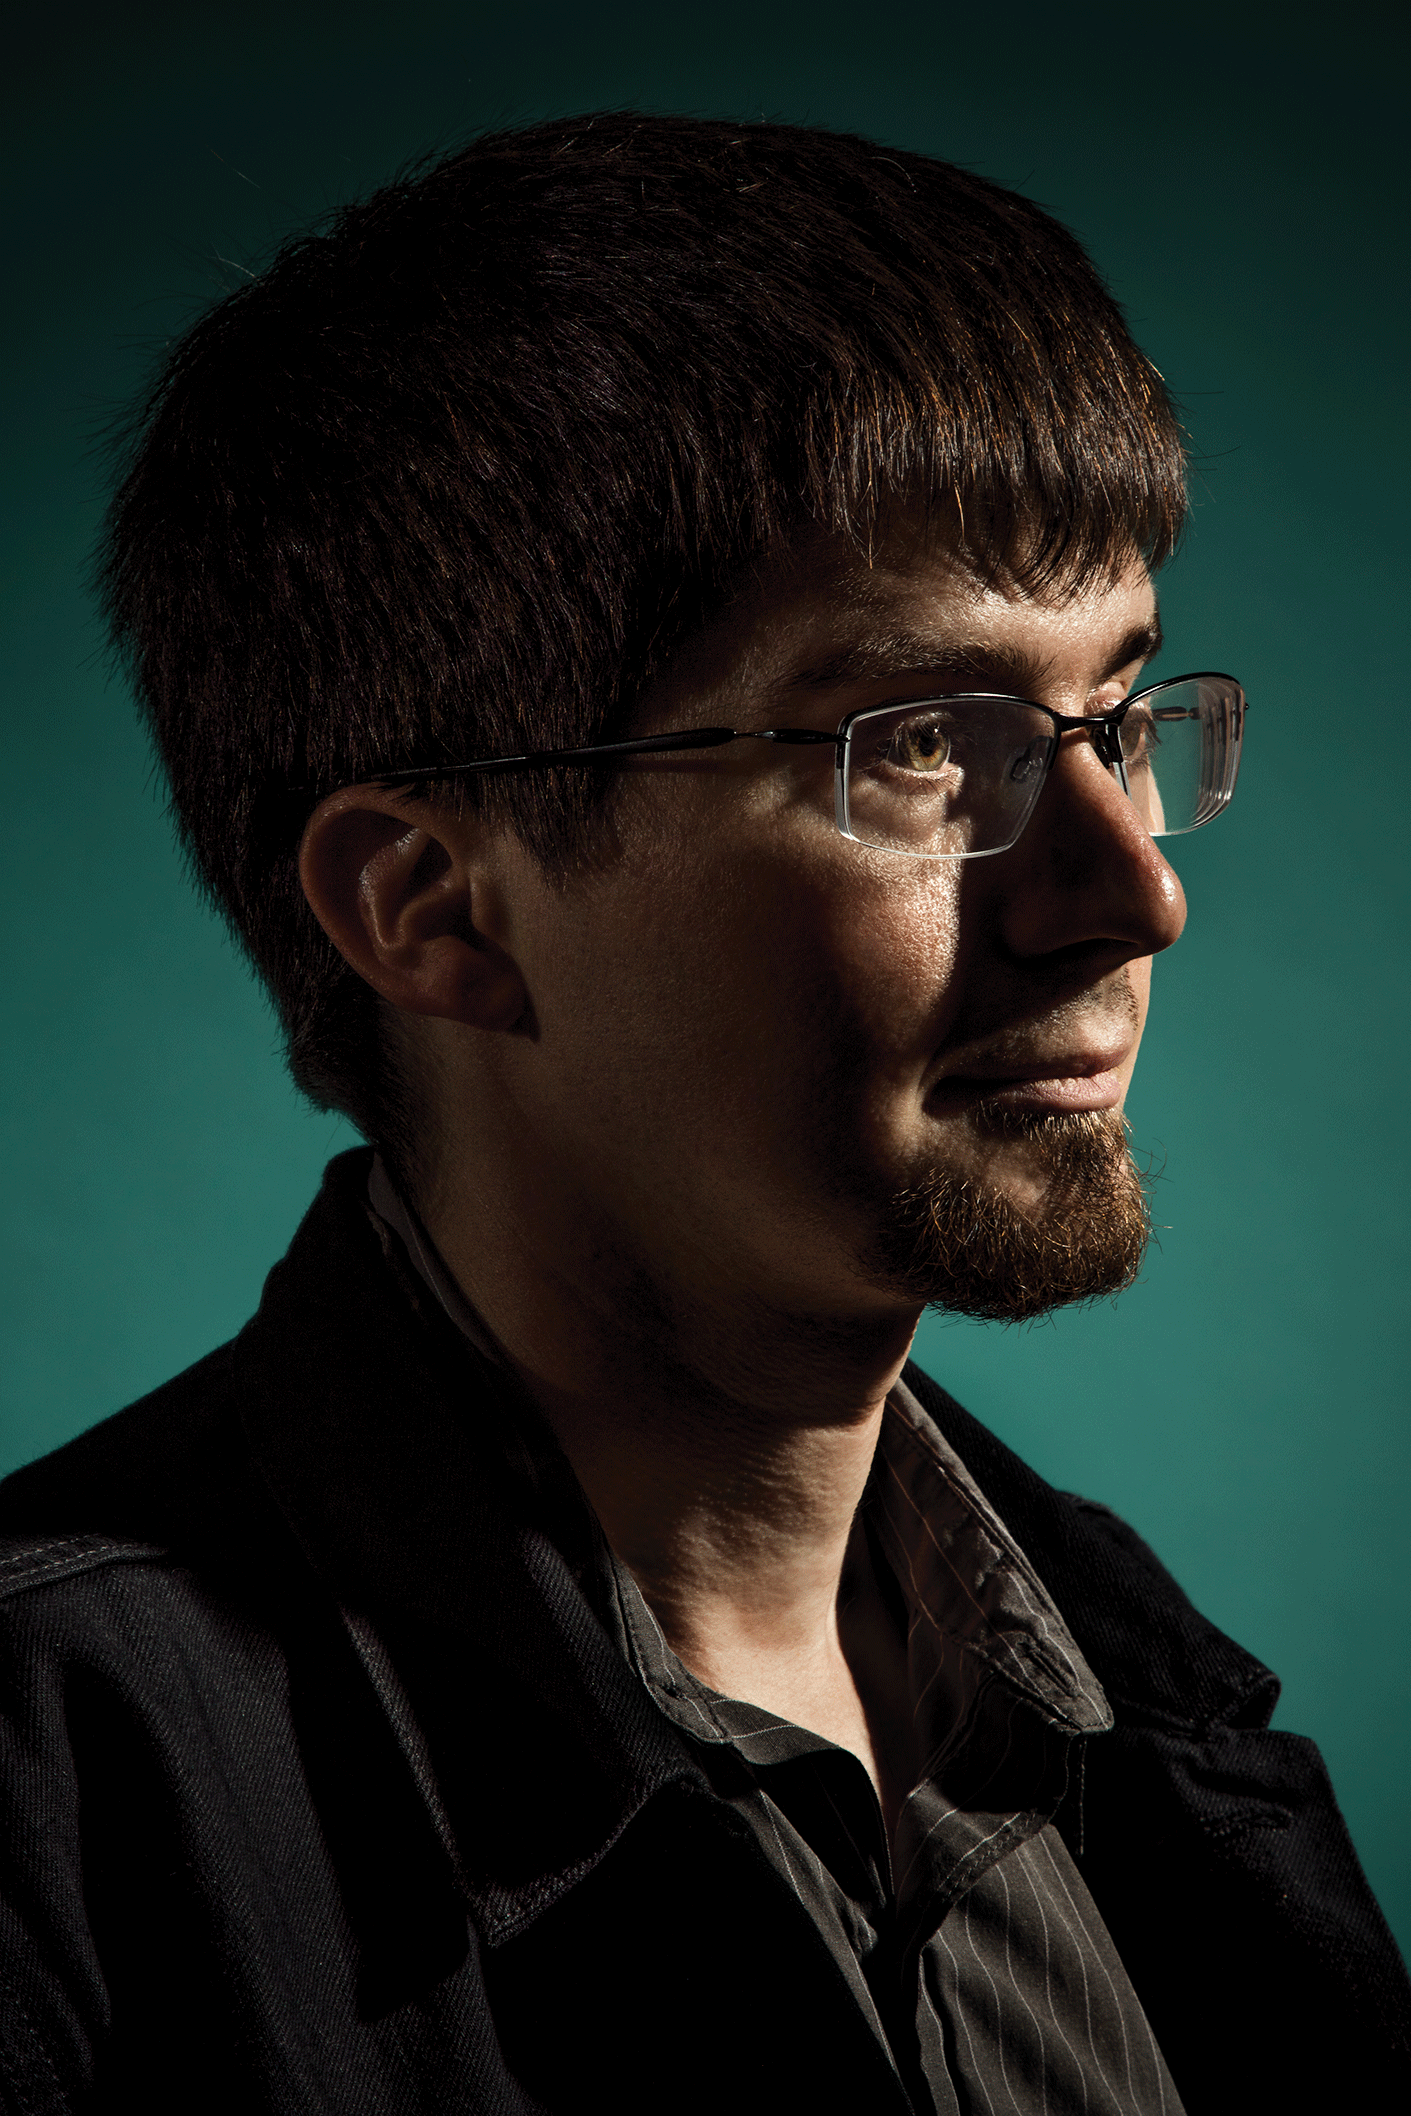
\includegraphics[width=0.25\textwidth]{figures/gan-goodfellow.png}
%         \label{fig:gan-ian-goodfellow}
%     \end{center}
%     \vspace{-20pt}
%     \caption{Ian Goodfellow. \\Fuente: \href{https://www.technologyreview.es/s/10016/el-senor-de-las-gan-el-hombre-que-dio-imaginacion-las-maquinas}{MIT Technology Review}}
% \end{wrapfigure}

Más adelante en el 2014 {Goodfellow} \ref{fig:gan-ian-goodfellow} presento la primera red neuronal \acrshort{gan} pura para la generación de imágenes mediante el enfrentamiento de una red neuronal generativa contra una red neuronal discriminante entrenadas con el mismo conjunto de datos \cite{goodfellow2014generative}.
Durante los proximos años se realizaron muchos aportes a las redes neuronales generativas, principalmente de paralelización de los calculos, técnicas de estabilización, generación condiciona, arquitecturas más eficientes, funciones de pérdidas más adecuadas, aplicaciones específicas (cambiar el estilo de pintura), redes apiladas, etc.
Fruto de todo ello {NVIDIA} en 2018 presento \gls{StyleGAN} \cite{karras2019stylebased} aunque publicaron el código en 2019 con fuertes mejoras.

\begin{figure}[H]
  \centering
  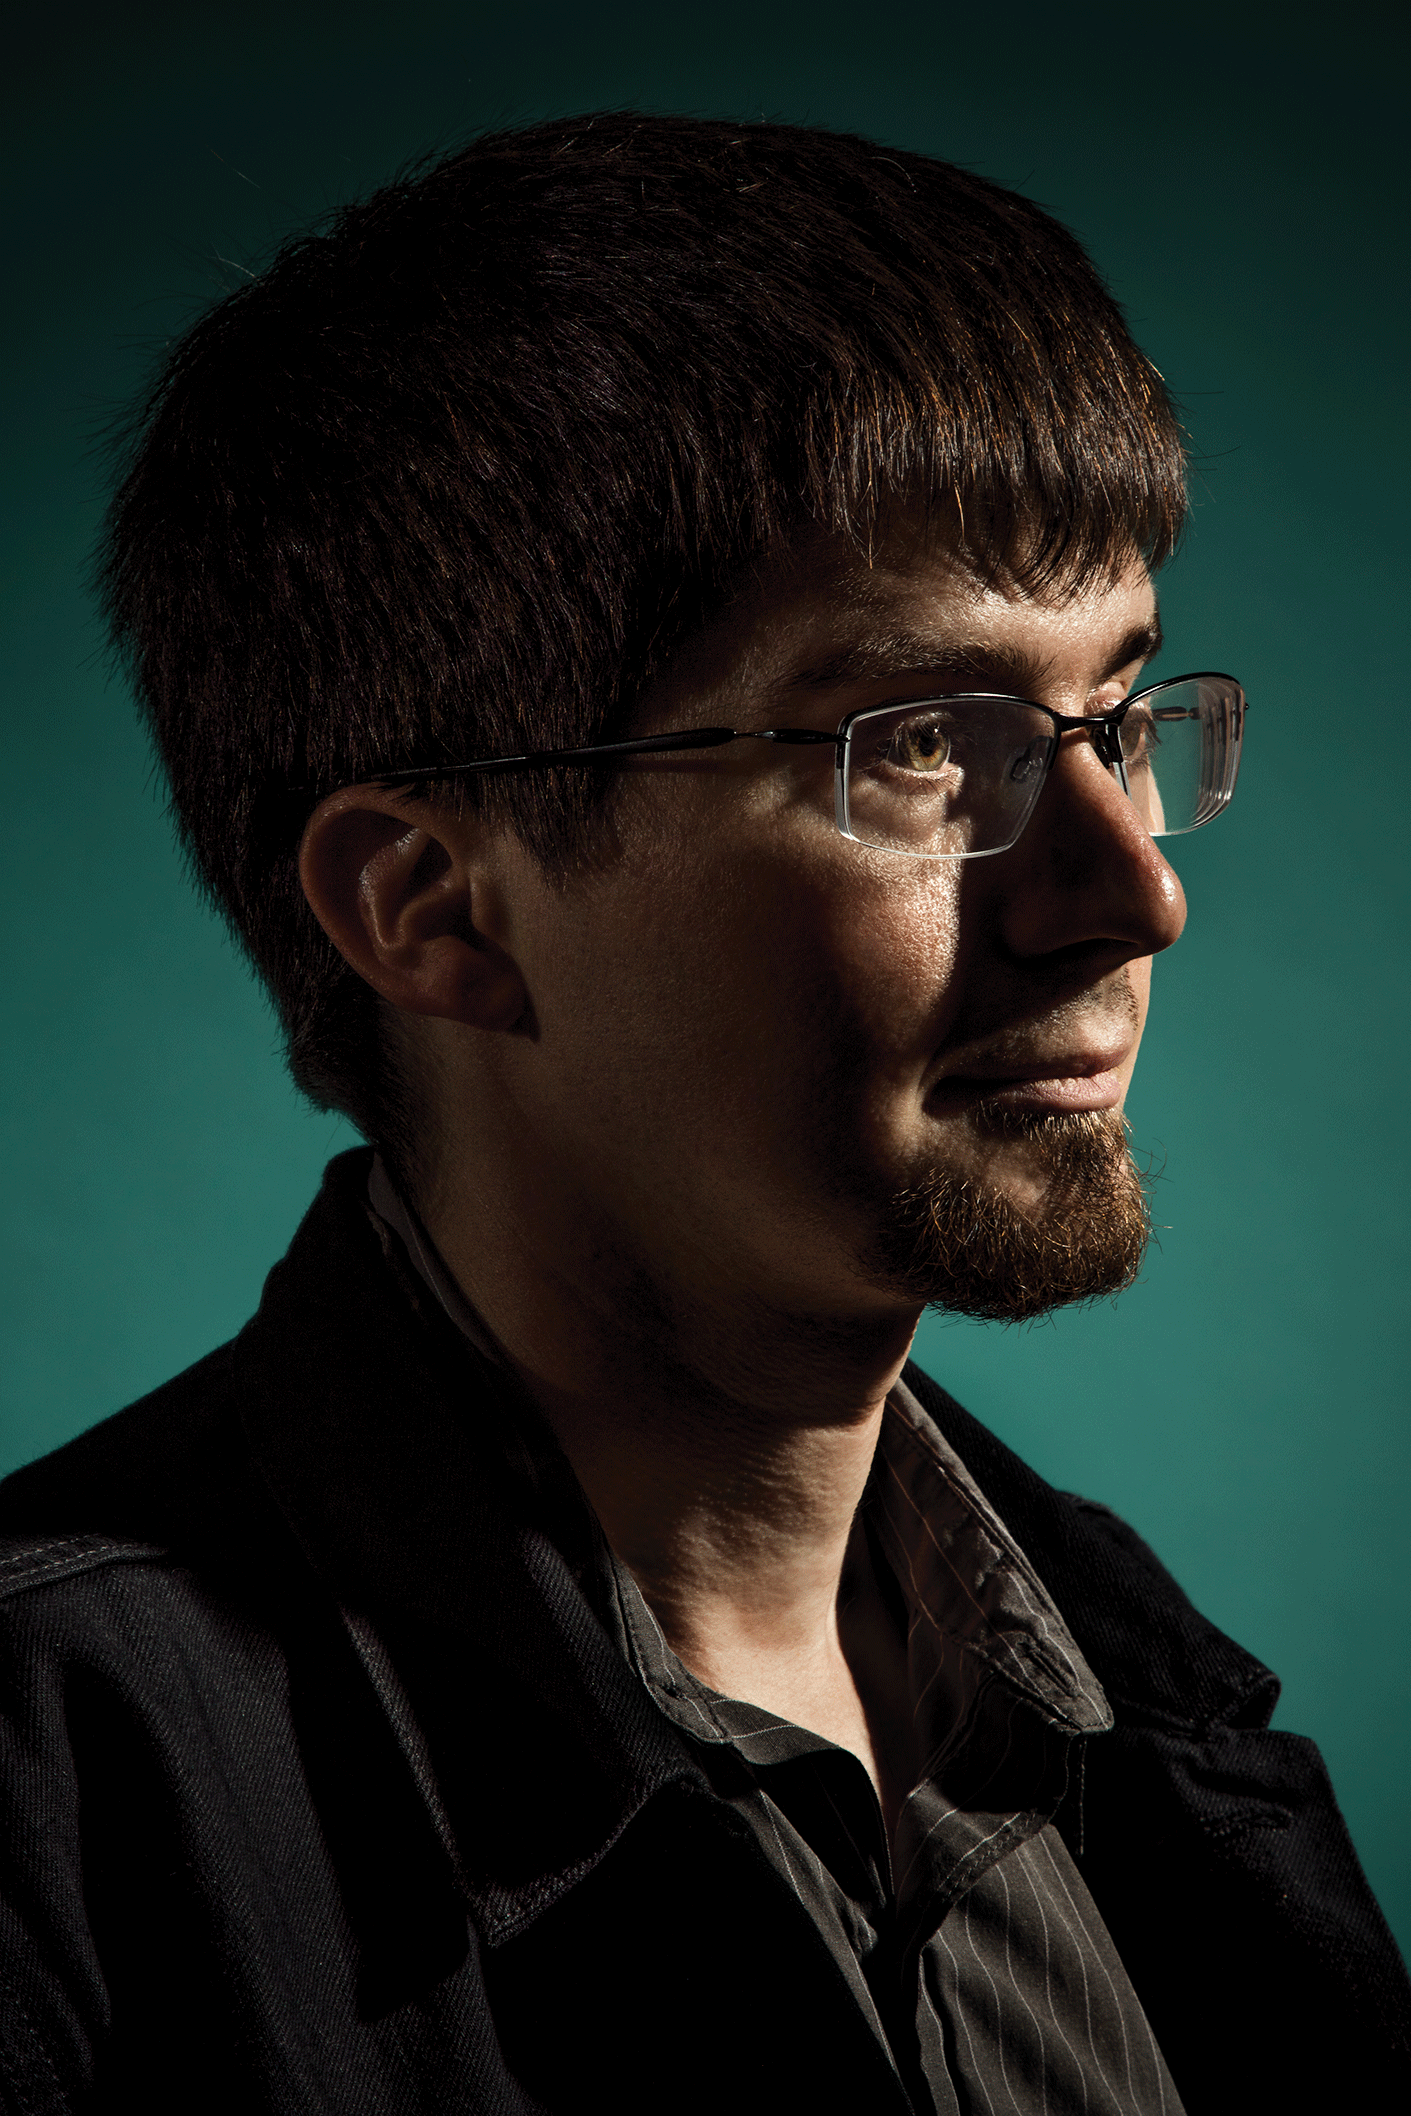
\includegraphics[width=0.2\textwidth]{figures/gan-goodfellow.png}
  \caption{Ian Goodfellow. \\Fuente: \href{https://www.technologyreview.es/s/10016/el-senor-de-las-gan-el-hombre-que-dio-imaginacion-las-maquinas}{MIT Technology Review}}
  \label{fig:gan-ian-goodfellow}
\end{figure}



\subsection{Defensas contra los ataques adversarios}

\subsection{Privacidad}

\subsection{Explicabilidad}

\subsection{Normativa y estándares}
% https://eur-lex.europa.eu/resource.html?uri=cellar:e0649735-a372-11eb-9585-01aa75ed71a1.0008.02/DOC_1&format=PDF
% https://eur-lex.europa.eu/resource.html?uri=cellar:e0649735-a372-11eb-9585-01aa75ed71a1.0008.02/DOC_2&format=PDF

% Segun la unión europea toda la seguridad es este apartado :ok: 
% (51) La ciberseguridad es fundamental para garantizar que los sistemas de IA resistan a las actuaciones de terceros maliciosos que, aprovechando las vulnerabilidades del sistema, traten de alterar su uso, conducta o funcionamiento o de poner en peligro sus propiedades de seguridad. Los ciberataques contra sistemas de IA pueden dirigirse contra elementos específicos de la IA, como los conjuntos de datos de entrenamiento (p. ej., contaminación de datos) o los modelos entrenados (p. ej., ataques adversarios), o aprovechar las vulnerabilidades de los elementos digitales del sistema de IA o la infraestructura de TIC subyacente. Por lo tanto, para asegurar un nivel de ciberseguridad adecuado a los riesgos, los proveedores de sistemas de IA de alto riesgo deben adoptar medidas adecuadas teniendo también en cuenta, cuando proceda, la infraestructura de TIC subyacente.









% https://www.youtube.com/@felipebravom



% Feb 1990: Generative Adversarial Networks / Curiosity Generative Adversarial Networks (GANs) have become very popular.[MOST] They were first published in 1990 in Munich under the moniker Artificial Curiosity. [AC90-20][GAN1] Two dueling NNs (a probabilistic generator and a predictor) are trying to maximize each other's loss in a minimax game.[AC](Sec. 1) The generator (called the controller) generates probabilistic outputs (using stochastic units[AC90] like in the much later StyleGANs[GAN2]). The predictor (called the world model) sees the outputs of the controller and predicts environmental reactions to them. Using gradient descent, the predictor NN minimizes its error, while the generator NN tries to make outputs that maximize this error: one net's loss is the other net's gain.[AC90] (The world model can also be used for continual online action planning.[AC90][PLAN2-3][PLAN])

% 4 years before a 2014 paper on GANs,[GAN1] my well-known 2010 survey[AC10] summarised the generative adversarial NNs of 1990 as follows: a "neural network as a predictive world modelis used to maximize the controller's intrinsic reward, which is proportional to the model's prediction errors" (which are minimized).

% The 2014 GANs are an instance of this where the trials are very short (like in bandit problems) and the environment simply returns 1 or 0 depending on whether the controller's (or generator's) output is in a given set.[AC20][AC][T22](Sec. XVII)

% Other early adversarial machine learning settings[S59][H90] were very different—they neither involved unsupervised NNs nor were about modeling data nor used gradient descent.

% The 1990 principle has been widely used for exploration in Reinforcement Learning[SIN5][OUD13] [PAT17][BUR18] and for synthesis of realistic images,[GAN1,2] although the latter domain was recently taken over by Rombach et al.'s Latent Diffusion, another method published in Munich,[DIF1] building on Jarzynski's earlier work in physics from the previous millennium[DIF2]  and more recent papers.[DIF3-5]

% In 1991, I published yet another ML method based on two adversarial NNs called Predictability Minimization for creating disentangled representations of partially redundant data, applied to images in 1996.

\section{Estado del arte}

\subsection{La ciencia de datos}
\subsection{La extracción del conocimiento}


% Fases de la extraccón del conocimiento 
% KDD
\subsection{Machine Learning}
\subsection{Deep Learning}
\subsection{Generative Adversarial Networks (GAN)}
